\section{Coding Theory}
Coding theory is a branch of mathematics that studies the properties of codes, in particular it focuses on the \textbf{error-detection} and \textbf{error-correction} capabilities of codes. 


\begin{figure}[h!]
  \centering
  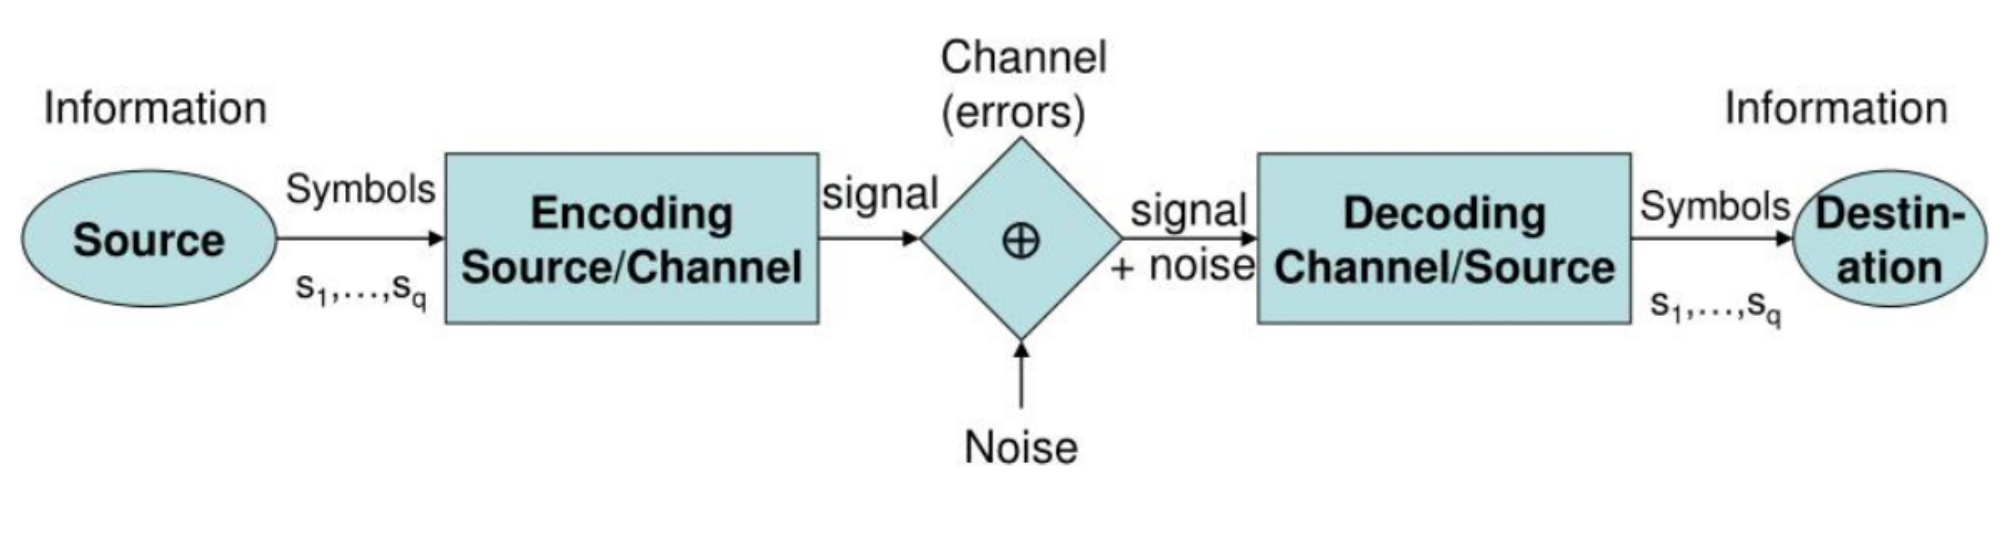
\includegraphics[width=1.2\textwidth]{images/section_4/coding_theory.png}
  \caption{Coding theory overview}
  \label{fig:coding-theory}
\end{figure}

\noindent
Each step shown in the figure above is crucial for the design and analysis of codes. The \textbf{encoding} step involves transforming the original message into a codeword using a specific encoding scheme. The \textbf{transmission} step is where the codeword is sent through a communication channel, which may introduce errors. The \textbf{decoding} step is where the received codeword is processed to recover the original message, and this is where error-detection and error-correction techniques come into play. \\
In the coding theory there are:

\begin{itemize}
    \item \textbf{$F$}: finite alphabet, which is the set of symbols used to construct codewords. For example, in binary codes, the alphabet is $\{0, 1\}$.
    \item \textbf{$m \in F^k$}: information word or message, which is the original data that we want to encode. It consists of $k$ symbols from the alphabet $F$.
    \item \textbf{$c \in F^n$}: codeword or input word, which is the encoded version of the message. It consists of $n$ symbols from the alphabet $F$, where $n \geq k$. 
    \item \textbf{$y \in F^n$}: received word or output word, which is the codeword that has been transmitted through the channel and may contain errors. It also consists of $n$ symbols from the alphabet $F$.
    \item \textbf{$\hat{c} \in F^n$} decoded word
    \item \textbf{$\hat{m} \in F^k$} decoded message
\end{itemize}

\subsection{Codewords}
For our purposes, we will consider \textbf{additive channels}, i.e., given c, y $\in F^n$, then
\begin{center}
    $y = c + e$
\end{center}
where $e$ is the error vector or error word. 
\medskip

\noindent
We define a (n, M)-code $C$ as  \underline{non empty subset of $F^n$ such that $|C| = n$} where $n$ is the \textbf{length} of the codewords and $M$ is the number of codewords in the code (\textbf{size}). \textit{(In this case the notation |C| doesn't mean "number of elemnts of C", but it means the leght of th vector)} \\
The quantity $k \coloneqq \log_{|F|} M$ is called the \textbf{dimension} or information length of the code and $R \coloneqq \frac{k}{n}$ is called the \textbf{rate} of the code.\\
The elements of $C$ are called \textbf{codewords}.

\subsubsection{Distances}

\begin{defBox}{Hamming Distance}
    GGiven x, y $\in F^n$, the Hamming distance between x and y is defined as the number of positions (coordinates) in which x and y differ.\\
    It is denoted as $d(x, y)$ 
\end{defBox}
\medskip

\begin{defBox}{Hamming Weight}
    AGiven x $\in F^n$, the Hamming weight of x is defined as the number of non-zero coordinates of x.\\
    It is denoted as $w(x)$
\end{defBox}
\medskip

\begin{defBox}{Minimum Distance}
    AGiven a (n, M)-code $C$, the minimum distance of $C$ is:
\begin{center}
    $d \coloneqq min\{d(c_1, c_2), \forall c_1, c_2 \in C, c_1 \neq c_2\}$
\end{center}
\noindent
\textit{Note that $d(c_1, c_2)$ is the Hamming distance between $c_1$ and $c_2$.}
\end{defBox}
\medskip

\noindent
The concept of minimum distance is crucial in coding theory, as it determines the error-detection and error-correction capabilities of the code. A code with a larger minimum distance can detect and correct more errors. Specifically, a code with minimum distance $d$ can detect up to $d-1$ errors and can correct up to $\lfloor \frac{d-1}{2} \rfloor$ errors (we will discuss the theorem later).
 (vedi Teorema~\ref{thm:error-detect-correct}).
\bigskip

\noindent
\textbf{Examples:}\\
Let us consider $F = \{0, 1\} = \mathbb{Z}_2 = \mathbb{F}_2$, we define the following code of leght $n = 3$ and size $M = 8$:
\begin{center}
    $C = \{000, 001, 010, 011, 100, 101, 110, 111\}$
\end{center}
\noindent
In this case, the dimension is $k = \log_2 8 = 3$, this means that all the bites are "information bits".\\
The minimum distance is $d = 1$. In this case we are not able to detect and correct any error.
\vspace{1 cm}

\noindent
Let us consider $F = \{0, 1\} = \mathbb{Z}_2 = \mathbb{F}_2$, we define the following code of leght $n = 6$ and size $M = 8$:
\begin{center}
    $C = \{000000, 001111, 110011, 111100, 101010, 010101, 011001, 100110\}$
\end{center}
\noindent
In this case, the dimension is $k = \log_2 8 = 3$ and the rate is $R = \frac{3}{6} = \frac{1}{2} = 0.5 $. This means that we have 3 information bits and 3 redundancy bits.\\
The minimum distance is $d = 2$. In this case we are able to detect 1 error but we are not able to correct any error.
\vspace{1 cm}

\noindent
Let us consider $F = \{0, 1\} = \mathbb{Z}_2 = \mathbb{F}_2$, we define the following code of leght $n = 9$ and size $M = 8$:
\begin{center}
    $C = \{000000000, 111111111, 000111111, 111000000, 001001001, 110110110, 010010010, 101101101\}$
\end{center}
\noindent
In this case, the dimension is $k = \log_2 8 = 3$ and the rate is $R = \frac{3}{9} = \frac{1}{3} \approx 0.33 $. This means that we have 3 information bits and 6 redundancy bits.\\
The minimum distance is $d = 3$. In this case we are able to detect 2 errors and we are able to correct 1 error.

\subsubsection{Conditions for correction and detection}
\begin{defBox}{Sphere of radius $r$}
    GGiven $x \in F^n$ and $r \in \mathbb{N}$, the sphere of radius $r$ and center $x$ is defined as:
    \begin{center}
        $S(x, r) \coloneqq \{x' \in F^n : d(x, x') \leq r\}$
    \end{center}  
\end{defBox}
\noindent
In an informal way, at the center of the sphere we have a codeword $c$, around $c$ we have all the possible words that we can obtain by introducing at most $r$ errors in $c$.\\
So, all that we can recieve by introducing at most $r$ errors starting from $c$.
\vspace{1 cm}

\noindent
\begin{propBox}{}{}
    \begin{itemize}
        \item A code $C$ detects $h_1$ errors if and only if $\forall c \in C$, we have $S_{h_1}(c) \cap C = \{c\}$
        \item A code $C$ corrects $h_2$ errors if and only if $\forall c_1, c_2 \in C$,  we have $S_{h_2}(c_1) \cap S_{h_2}(c_2) = \emptyset$
    \end{itemize}
\end{propBox}

\noindent
First proposition, underline that in each sphere of radius $h_1$ and center $c$ there is only $c$ itself, so just one codeword.\\
Second proposition, underline that two different codewords $c_1$ and $c_2$ have two spheres of radius $h_2$ that do not intersect, so they are disjoint.
\vspace{1 cm}

\noindent
\begin{thmBox}{Error Detection and Correction Capabilities}
    AGiven a code $C$ with minimum distance $d$, then $C$ detects up to $d-1$ errors and corrects up to $\lfloor \frac{d-1}{2} \rfloor$ errors.
    \label{thm:error-detect-correct}
\end{thmBox}



\subsection{Linear codes}
This sub-section is about "how contruct codes". In particular, we will focus on \textbf{linear codes}, which are a special class of codes that have a linear structure.\\
We will always consider $F = \mathbb{F}_q$ a finite fiels with q elements, where $q$ is a prime or a power of a prime.
\medskip

\begin{defBox}{Linear Code}
    AA code $C$ with parameters (n, M, d) is called linear if $C$ is a linear subspace of $F^n_q$ over $F_q$.
\end{defBox} 

\noindent
For linear codes, we use the notation [n, k, d] to denote a linear code of length n, dimension k and minimum distance d.\\
The difference (n - k) is called the \textbf{redundancy} of the code, and it represents the number of redundancy bits added to the information bits to form the codewords.
\bigskip

\noindent
\textbf{Remark:}
In a linear code, the linear combination of two codewords is still a codeword.
\vspace{1 cm}

\noindent
\textbf{Example:}
Let us construct a linear code of dimension k = 2 over $\mathbb{F}^5_2$.\\
It is sufficient to take two linearly indipendet vectors in $\mathbb{F}^5_2$, for example:
\begin{center}
    $c_1 = (1, 0, 1, 1 , 1)$\\
    $c_2 = (1, 1, 1, 1, 0)$
\end{center}
\noindent
and thus all the codewords are $a_1 c_1 + a_2 c_2 \forall a_1, a_2 \in \mathbb{F}_2$, so we have:\\
\begin{center}
    $C = \{00000, 10111, 11110, 01001\}$
\end{center}
\noindent
We can observe that the minimum distance is $d = 2$
\vspace{1 cm}


\noindent
\textbf{Remark:}
For linear code $C$, we can observe that the null vector 0 = (000...0) is always a codeword and moreover
\begin{center}
    $d(c_1, c_2) = d(c_1 - c_2, 0)$
\end{center}
\noindent
for all $c_1, c_2 \in C$, and thus
\begin{center}
    $ d = \min_{\substack{x \in C \\ x \neq 0}} w(x) $
\end{center}
\noindent
In general, if M is the size of a code, then, in order to evaluete d, we neeed to evaluate the Hamming distance between all the pairs of elements of C, i.e., $\binom{M}{2} \simeq M^2$.\\
For a linear code, it is sufficient to perform M-1 cheks.

\subsubsection{Generator matrix}
In general a matrix is a rectangular array of numbers, symbols, or expressions, arranged in rows and columns. In coding theory, we use matrices to represent linear codes, to perform encoding and decoding operations or to memorize the codewords of a linear code.
\medskip
For our purposes, we discuss a lot about the \textbf{generator matrix}.

\begin{defBox}{Generator Matrix}
    AGiven a linear code $C$ with parameters [n, k, d], a generator matrix for $C$ is a k x n matrix $G$ whose rows form a basis for $C$. 
\end{defBox}

\noindent
All the codewords can be obtained using the generator matrix with all the information words, which are all the elements of $\mathbb{F}_q^k$, i.e.,
\begin{center}
    $C = \{mG : m \in \mathbb{F}_q^k\}$
\end{center}
\noindent
Thus, an information word m is encoded into a codeword $c = mG$.\\
A linear code is completely determined by G, i.e., $kn$ elements of $F_q$ are sufficient to fully describe a code $C$ that contains $q^k$ vectors of length n (i.e., $q^k n$ elements of $F_q$).
\vspace{1 cm}

\noindent
A $k \times n$ generator matrix $G$ is called \textbf{systematic} if ot has the form
\begin{center}
    $G = (I|A)$
\end{center}
\noindent
where $I$ is the $k \times k$ identity matrix and $A$ is a $k \times (n-k)$ matrix.\\
A linear conde allows a systematic generator matrix if and only if the first $k$ columns of any generator matrix are linearly independent.\\
If $G$ is a systematic generator matrix, we can observe that given an information word $m = (m_1, m_2, ..., m_k) \in \mathbb{F}_q^k$ an information word, then
\begin{center}
    $c = mG = (m_1, m_2, ..., m_k | p_1, p_2, ..., p_{n-k}) \in \mathbb{F}_q^n$ 
\end{center}
i.e., the first $k$ elements of a codeword are the elements of the information word.\\
This means that it is immediate to recover the information word from the codeword.

\vspace{1 cm}
\noindent
We define the \textbf{dot product} in $\mathbb{F}_q^n$ as follows:
\begin{center}
    $x \cdot y \coloneqq x_1 y_1 + x_2 y_2 + ... + x_n y_n$
\end{center}
\noindent
for all $x , y \in \mathbb{F}_q^n$

\begin{defBox}{Dual Code}
    AGiven a linear code $C \in \mathbb{F}_q^n$, the dual code of $C$ is defined as:
    \begin{center}
        $C^\perp \coloneqq \{x \in \mathbb{F}_q^n : x \cdot y = 0, \forall y \in C\}$
    \end{center}

\noindent
The generator matrix $H$ of $C^\perp$ is called the \textbf{parity-check matrix} of $C$.
\end{defBox}
\medskip

\begin{propBox}{}{}
    Given a recieved word $y \in \mathbb{F}_q^n$, we have
    \begin{center}
        $y \in C \iff yH^T = 0$
    \end{center}
\end{propBox}
\medskip

\begin{propBox}{}{}
   If $G = (I_k | A)$, then $H = (-A^T | I_{n-k})$
\end{propBox}
\medskip

\noindent
\textbf{Example:}
Let us consider linear code $C$ with generator matrix
\begin{center}
    \[
    \begin{pmatrix}
        1 & 0 & 0 & 0 & 1 & 1 & 1 \\
        0 & 1 & 0 & 0 & 0 & 1 & 1 \\
        0 & 0 & 1 & 0 & 1 & 0 & 1 \\
        0 & 0 & 0 & 1 & 1 & 1 & 0\\
    \end{pmatrix}
    \]
\end{center}
\noindent
Thus $C$ is a linear code of length $n = 7$, dimension $k = 4$.\\
We can observe that
\begin{center}
    $C = \{(m_1, m_2, m_3, m_4, m_1 + m_3 + m_4, m_1 + m_2 + m_4, m_1 + m_2 + m_3) : m_i \in \mathbb{F}_q\}$
\end{center}
\noindent
and
\begin{center}
    $H = \begin{pmatrix}
        1 & 0 & 1 & 1 & 1 & 0 & 0 \\
        1 & 1 & 0 & 1 & 0 & 1 & 0 \\
        1 & 1 & 1 & 0 & 0 & 0 & 1 \\
    \end{pmatrix}$
\end{center}
\noindent
from which we obtain that $y = (y_1, y_2, ...., y_7) \in C$ if and only if
\[
\begin{cases}
    y_1 + y_3 + y_4 + y_5 = 0 \\
    y_1 + y_2 + y_4 + y_6 = 0 \\
    y_1 + y_2 + y_3 + y_7 = 0
\end{cases}
\]    

\subsubsection{Identification of errors}
As already said, one of the main goals of coding theory is to identify and correct errors.\\
To do this, we have to define the \textbf{nearest-codeword decoding}. It consists in: given a received word $y \in \mathbb{F}_q^n$, find a codeword $c \in C$ that minimizes the Hamming distance $d(y, c)$ or equivalently find an error $e \in \mathbb{F}_q^n$ of minimum Hamming weight s.t. $y - e \in C$.
\medskip

\noindent
Let $C$ be a linear [n, k, d]-code and let $H$ be a parity-check matrix for $C$. We define the function $s : \mathbb{F}_q^n \rightarrow \mathbb{F}_q^{n-k}$ such that
\begin{center}
    $s(y) = yH^T$
\end{center}
\noindent
The function $s$ is called the \textbf{syndrome} of $y$.\\
\vspace{1 cm}

\noindent
Given a recieved word $y = c + e$, we have that $s(y) = s(e)$.\\
Thus, given a recieved word y, the idea to detect and correct errors is the following:

\begin{algorithm}
\begin{algorithmic}[1]

\State Pre-compute the syndrome of all possible errors that the linear code is able to correct
\State evaluate the syndrom $s(y)$
\State if $s(y) = 0$, then there are no errors (we recieved a codeword)
\State if $s(y) \neq 0$, then we have an error, and we can identify the error by looking at the pre-computed syndromes; if $s(y) = s(e)$ for some error $e$, then correcr $y$ with $y-e$ 

\end{algorithmic}
\end{algorithm}

\noindent
\textbf{Example:}
Let $C$ be a linear [4, 3]-code over $\mathbb{F}_3 = \mathbb{Z}_3 = \{0, 1, 2\}$ with parity-check matrix
\begin{center}
    $H = \begin{pmatrix}
        1 & 1 & 0 & 2 \\
        0 & 2 & 1 & 2 \\
    \end{pmatrix}$
\end{center}
\noindent
Thus, the linear code is defined by the following equations:
\[\begin{cases}
    x_1 = -x_2 + x_4 \\
    x_3 = x_2 + x_4
\end{cases}\]
\noindent
and then
\begin{center}
    $C = \{(a+b, -a, -a+b, b) : a, b \in \mathbb{Z}_3\}$
\end{center}
\noindent
We can check that the minimum distance is $d = 3$, hence we are albe ro detect 2 errores and to correct only 1.
\smallskip

\noindent
The possible errors that we are able to correct are
\begin{center}
    $e_1 = (1, 0, 0, 0)$, $e_2 = (0, 1, 0, 0)$, $e_3 = (0, 0, 1, 0)$, $e_4 = (0, 0, 0, 1)$, $2e_1 = (2, 0, 0, 0)$, $2e_2 = ( 0, 2, 0, 0)$, $2e_3 = (0, 0, 2, 0)$, $2e_4 = (0, 0, 0, 2)$
\end{center}
\noindent
Thus, if we receive the word $y = (2, 1, 2, 1)$, we evaluate the syndrome 
\begin{center}
    $s(y) = yH^T = (2, 1, 2, 1) \begin{pmatrix}
        1 & 0 \\
        1 & 2 \\
        0 & 1 \\
        2 & 2 \\
    \end{pmatrix} = (2, 0)$
\end{center}
\noindent
since is different from 0, we check the pre-computed syndromes of the possible errors and we find that it is equal to $s(2e1)$

\subsubsection{Goppa Codes}
A (binary) Goppa code is a linear code defined by menas of a particular parity check matrix (and consequently a generator matrix) with a fast method for 'decoding', i.e., for correctiong errors.\\
Given $\alpha_1, \alpha_2, ....., \alpha_n \in \mathbb{F}_{2^m}$ and $g(x) \in \mathbb{F}_{2^m} [x]$ irreducible of degree $t$. Define a linear code $C$ with parity-check matrix:
\begin{center}
    $H = \begin{pmatrix}
        1 & 1 & ... & 1 \\
        \alpha_1 & \alpha_2 & \alpha_3 & ... & \alpha_n \\
        \alpha_1^2 & \alpha_2^2 & \alpha_3^2 & ... & \alpha_n^2\\
        ... & ... & ... & ... & ... \\
        \alpha_1^{t-1} & \alpha_2^{t-1} & \alpha_3^{t-1} & ... & \alpha_n^{t-1} \\
        \end{pmatrix} \cdot D $
\end{center}
\noindent
where D is a diagonal matrix where in the diagonal there are the elements $\frac{1}{g(\alpha_i)}$ and $t$ is the dedree of $g(x)$
\bigskip

\noindent
if $g(x)$ is an irreducible polynomial, then the minimum distance of the Goppa code is at least $2t + 1$. Moreover, the syndrome of a word $y$ has a very nice closed form:
\begin{center}
    $s(y) = (s_0, s_1, ..., s_{t-1})$
\end{center}
\noindent
where $s_0, s_1, ..., s_{t-1}$ are the coefficients of the polynomial
\begin{center}
    $\sum_{i=1}^n \frac{y_i}{x - \alpha_i} \mod g(x)$.
\end{center}
\medskip

\noindent
For performing the correction of errors occured in a received word $y = c + e$, its \textbf{error locating polynomial is used}
\begin{center}
    $\sigma(x) = \prod_{i : e_i \neq 0} (x - \alpha_i)$
\end{center}
\noindent
where the product ranges over the indexs $i$ such that $e_i \neq 0$.\\
Thus, the main problem is to evaluate the polynomial $\sigma(x)$, associated to a given received word.\\
For this reason, we can use the \textbf{Patterson algorithm}, which is an efficient algorithm for finding the error locating polynomial $\sigma(x)$ given the syndrome $s(y)$.


\begin{algorithm}
\caption{Patterson Algorithm }
\begin{algorithmic}[1]

\State Evaluate the syndrome $s(y)$ and denote by $s(X)$ the corresponding polynomial
\State Find $h(X)$ s.t. $s(X)h(X) \equiv 0 \mod g(X)$; if $h(X) = 0$, then output $\sigma(X) = 1$
\State Evaluate $d(X)$ s.t. $d(X)^2 \equiv h(X) + X \mod g(X)$
\State Find $a(X)$ and $b(X)$ s.t. $d(X)b(X) \equiv a(X) \mod g(X)$
\State Set $\sigma(X) = a(X)^2 + X b(X)^2X$
\State Use $\sigma(X)$ to find the error locations
\end{algorithmic}
\end{algorithm}

\subsubsection*{Summary}
Let $C$ be a (n,M,d)-code, able to detect d-1 errors and to correct
$t = [(d-1)/2]$ errors. Let y be a received word.
\begin{itemize}
    \item If C is not structured, for detecting the errors, we need to compare y with all the codewords and, if $y \notin C$, we can correct the errors with the idea of the nearest-codeword decoding.
    \item If C is a linear code, for detecting the errors, it is sufficient to evaluate the syndrome and, if it is not zero, we can correct the errors comparing this value with the pre-computed syndromes of all possible errors
    \item If C is a Goppa code, we detect the errors as a classical linear code and, if there are errors, we correct them with the Patterson algorithm, which is more efficient than the syndorme method when we need to correct many errors.
\end{itemize}


